\documentclass[aspectratio=169]{beamer}
\usetheme{gotham}
\usepackage{standalone}
\gothamset{colorset=anthracite}
\gothamset{background=transparent}
\gothamset{
  progressbar position=foot,
  progressbar style=rounded box,
  progressbar advancement=brlt,
  numbering=totalframenumber
}
\usepackage{tikz}
\tikzstyle{step} = [circle, minimum size=1.2cm, draw=black, fill=blue!20, text centered]
\tikzstyle{arrow} = [thick,->,>=stealth]
\usepackage{pgfplots}
\pgfplotsset{compat=1.18}
\usepackage{tabularray}
\UseTblrLibrary{booktabs}
\usepackage{changepage}
\usepackage{fancyvrb}
\usepackage{listings}
\usepackage{xcolor}
\definecolor{codeback}{rgb}{0.90,0.91,0.92}
\definecolor{codebackdark}{rgb}{0.10,0.11,0.12}
\newcommand{\famName}[1]{\textsc{#1}}
\newcommand{\themename}{\textbf{\textsc{Gotham}}}
\usepackage[style=authoryear,backend=biber]{biblatex}
%\addbibresource{../ref.bib}

\usepackage{hyperref} % for next buttons 

% Code listing style
\lstset{
  backgroundcolor=\color{codeback},
  basicstyle=\ttfamily\tiny,
  breaklines=true,
  frame=single,
  rulecolor=\color{gray!40},
  tabsize=2,
  showstringspaces=false,
  keywordstyle=\color{blue!70!black}\bfseries,
  commentstyle=\color{gray},
  stringstyle=\color{orange!80!black},
  language=Python
}

\defbeamertemplate{title page}{}{
    \centering
    {\huge \inserttitle} \\[1em]
    {\large \insertauthor} \\[1em]
    {\insertdate}
}

\title{Mental health: data explainer (internal use only)}
\author{Allegra Saggese for Professors Galina Hale, Hanna Kim}
\date{\today}

%%%%%%%%%% BEGIN DOC %%%%%%%%%%%
\begin{document}

\begin{frame}
  \titlepage
\end{frame}

% ─────────────────────────────────────────────────────────────────────────────
%  SECTION 1: DATA OVERVIEW
% ─────────────────────────────────────────────────────────────────────────────

\section{Data sources}

\begin{frame}{Summary of data sources (1/2)}
\begin{itemize}
    \item \textbf{USDA NASS agriculture data:} Count of county-level CAFO operations classified as Small/Medium/Large by animal (hogs, chickens, cattle). Census years only: 2002, 2007, 2012, 2017. Pulled via USDA Quick Stats API.
    \item \textbf{USDA FSIS data:} Count of federally-inspected slaughterhouses and meat processing plants by size bucket and animal type at county-level. Source: FOIA request. Geographic recovery via HUD ZIP-to-FIPS crosswalk.
    \item \textbf{CDC mortality data:} Deaths of despair (drug overdose + suicide + alcohol) at county-level from CDC WONDER, annual. Crude rates suppressed for counties with $<10$ deaths.
\end{itemize}
\end{frame}


\begin{frame}{Summary of data sources (2/2)}
\begin{itemize}
    \item \textbf{County Health Rankings (CHR) data:} Self-reported survey measures of mental health and health behaviors at county-level. Annual coverage from \textasciitilde2004. Variable selection based on cross-year availability.
    \item \textbf{Crime data:} FBI UCR incident-level arrests collapsed to FIPS-year. Violent crime subset selected by research team.
    \item \textbf{Population and geographic data:} US Census Bureau county population (1990--2024). NCHS urban-rural classification (6-level) used to define the main analytical sample.
\end{itemize}
\end{frame}

% ─────────────────────────────────────────────────────────────────────────────
%  SECTION 2: FILE LOCATIONS
% ─────────────────────────────────────────────────────────────────────────────
\section{Key files (csv)}

\begin{frame}{File locations: Shared directory structure}

All data lives in the shared \texttt{\textasciitilde/Dropbox/Mental/} folder. \textbf{Do not move or rename top-level folders, as the scripts are set to run from the dropbox structure.}

\vspace{0.5em}

Starting with the raw data files: 
\textbf{Raw inputs} (\texttt{Data/raw/})
\begin{itemize}\small
    \item \texttt{cdc/} — CDC WONDER mortality CSVs \hyperlink{0c}{\beamerbutton{cleaning script}}
    \item \texttt{crime/total-v1/} — FBI UCR (pre-assembled) annual CSVs
    \hyperlink{0d}{\beamerbutton{cleaning script}}
    \item \texttt{fips/} — FIPS crosswalk (county-year key) 
    \item \texttt{mental/} — County Health Rankings CSVs \hyperlink{0c}{\beamerbutton{cleaning script}}
    \item \texttt{nchs/} — \texttt{NCHSurb-rural-codes.csv} \hyperlink{0e}{\beamerbutton{details}}
    \item \texttt{population/} — Census population CSVs \hyperlink{0a}{\beamerbutton{details}}
    \item \texttt{usda/} — USDA agriculture census \texttt{.dta} fallback files \hyperlink{0b}{\beamerbutton{cleaning script}}
    \item \texttt{fsis/} — FSIS (FOIA-requested) inspection CSVs \hyperlink{0f}{\beamerbutton{cleaning script}}
\end{itemize}

\end{frame}


\begin{frame}{File locations: Shared directory structure}

Clean outputs are the cleaned versions of each input source. If source was stored across multiple files (csvs, .dta files), the clean output contains the consolidated year-county version of the data. 

\vspace{0.5em}

Next we have interim, but organized \textbf{clean outputs} (\texttt{Data/clean/})
\begin{itemize}\small
    \item \texttt{YYYY-MM-DD\_population\_full.csv}
    \item \texttt{YYYY-MM-DD\_cafo\_ops\_by\_size\_compact.csv}
    \item \texttt{YYYY-MM-DD\_mh\_mortality\_fips\_yr.csv}
    \item \texttt{YYYY-MM-DD\_mentalhealthrank\_full.csv}
    \item \texttt{YYYY-MM-DD\_cdc\_county\_year\_deathsofdespair.csv}
    \item \texttt{YYYY-MM-DD\_crime\_fips\_level\_final.csv}
    \item \texttt{YYYY-MM-DD-rural-key.csv}
    \item \texttt{YYYY-MM-DD\_fsis\_county\_year\_...\_summary.csv}
\end{itemize}

\end{frame}


\begin{frame}{Data/clean/ files: unit of observation \& contents (1/4)}
\begin{tblr}{
  colspec = {Q[l,2.7cm] Q[l,1.7cm] Q[l,1.5cm] Q[l,6.4cm]},
  hlines, vlines,
  row{1} = {font=\bfseries\small},
  row{2-Z} = {font=\footnotesize},
}
File & Unit of obs. & Years & Descriptor + key variables \\
\texttt{population\_full.csv} & county-year & 1990--2024 & Annual Census population, 4 vintages spliced \& FIPS-expanded. \textbf{Raw:} \texttt{population}, \texttt{state}/\texttt{division}/\texttt{region}. 100\% coverage --- panel denominator. \\
\texttt{fips\_full.csv} & county-year (ref.) & 1990--2024 & FIPS$\leftrightarrow$county-name crosswalk, expanded to annual rows per census-decade vintage. \textbf{Raw} reference table for key normalization (not merged into panel). \\
\end{tblr}
\end{frame}


\begin{frame}{Data/clean/ files: unit of observation \& contents (2/4)}
\begin{tblr}{
  colspec = {Q[l,2.7cm] Q[l,1.7cm] Q[l,1.5cm] Q[l,6.4cm]},
  hlines, vlines,
  row{1} = {font=\bfseries\small},
  row{2-Z} = {font=\footnotesize},
}
File & Unit of obs. & Years & Descriptor + key variables \\
\texttt{cafo\_ops\_by\_} \texttt{size\_compact.csv} & county $\times$ year $\times$ commodity (5 types) & 2002, 2007, 2012, 2017, 2022 & USDA NASS operation counts by size. \textbf{Raw:} \texttt{small}, \texttt{medium}, \texttt{large}, \texttt{bin\_sum}, \texttt{total\_heads}. \textbf{Derived:} \texttt{any\_large\_cafo}, \texttt{any\_medium\_or\_large\_cafo} (presence flags). \\
\texttt{cdc\_county\_year\_} \texttt{deathsofdespair.csv} & county-year & 2000--2020 & CDC WONDER deaths of despair (drug overdose + suicide + alcohol). \textbf{Raw:} \texttt{deaths}, \texttt{population}, \texttt{crude\_rate}, \texttt{crude\_rate\_raw}, \texttt{is\_unreliable}, \texttt{pct\_of\_total\_deaths}. Crude rate suppressed $<10$ deaths. \\
\end{tblr}
\end{frame}


\begin{frame}{Data/clean/ files: unit of observation \& contents (3/4)}
\begin{tblr}{
  colspec = {Q[l,2.7cm] Q[l,1.7cm] Q[l,1.5cm] Q[l,6.4cm]},
  hlines, vlines,
  row{1} = {font=\bfseries\small},
  row{2-Z} = {font=\footnotesize},
}
File & Unit of obs. & Years & Descriptor + key variables \\
\texttt{crime\_fips\_level\_} \texttt{final.csv} & county-year & 1991--2021 & FBI UCR violent-crime incident counts, collapsed from precinct level. \textbf{Raw:} 12 incident-type counts (\texttt{aggravated\_assault}, \texttt{rape}, \texttt{simple\_assault}, etc.). \textbf{Derived:} \texttt{total\_incidents} (row sum). \\
\texttt{mentalhealthrank\_} \texttt{full.csv} & county-year & 2010--2023 & County Health Rankings survey, $\sim$50 measures. \textbf{All raw} as reported by CHR: \texttt{*\_raw\_value}, \texttt{*\_numerator}, \texttt{*\_denominator}, \texttt{*\_ci\_high/low}. (Per-100k \& count-imputed versions built later, in the panel.) \\
\end{tblr}
\end{frame}


\begin{frame}{Data/clean/ files: unit of observation \& contents (4/4)}
\begin{tblr}{
  colspec = {Q[l,2.7cm] Q[l,1.7cm] Q[l,1.5cm] Q[l,6.4cm]},
  hlines, vlines,
  row{1} = {font=\bfseries\small},
  row{2-Z} = {font=\footnotesize},
}
File & Unit of obs. & Years & Descriptor + key variables \\
\texttt{...-rural-key.csv} & county-year & 2000--2023 & NCHS urban-rural codes, forward-filled from 4 base years (1990/2006/2013/2023). \textbf{Raw:} \texttt{nchs\_code}, \texttt{nchs\_label}, \texttt{cbsa\_pop}, \texttt{county\_pop}. \textbf{Derived:} sample filter $\rightarrow$ becomes \texttt{rural} in the panel. \\
\texttt{..fsis\_county\_} \texttt{year\_..summary\_..csv} & county-year & 2017--2026 & FSIS-regulated establishment counts by type \& size bucket; FIPS recovered via HUD ZIP crosswalk. \textbf{All raw} counts: \texttt{n\_unique\_establishments}, \texttt{n\_meat\_slaughter\_establishments}, \texttt{n\_size\_bucket\_1}--\texttt{5}, etc. \\
\end{tblr}
\end{frame}


\begin{frame}{File locations: Complete panel}

{\small \textbf{Merged panel:} (\texttt{Data/merged/}): \texttt{YYYY-MM-DD\_full\_merged.csv} — the main analysis file. Always use the most recent date prefix.}

\vspace{.05em}

\texttt{script1c-merge-dataclean.py} is the only script that writes \texttt{YYYY-MM-DD\_full\_merged.csv}, and that file is the \textit{one and only analysis panel}. Export on line 794-797. Everything in the set of \texttt{script2*} reads this file and produces figures or quality assurance outputs. There is no modification or re-export of the panel. \hyperlink{execution-order}{\beamerbutton{script pipeline details}}
\end{frame}




\begin{frame}{File locations: Where (and what) are the key files?}
\begin{tblr}{
  colspec = {Q[l,3cm] Q[l,5.8cm] Q[l,3cm]},
  hlines, vlines,
  row{1} = {font=\bfseries\small},
  row{2-Z} = {font=\small},
}
Use Case & File (assume \texttt{YYYY-MM-DD} prefix)  & Location \\
Full panel (all years) & \texttt{\_full\_merged.csv} & \texttt{Data/merged/} \\
2005--2010 slice & \texttt{\_full\_merged\_2005\_2010.csv} & \texttt{Data/merged/} \\
2010--2020 slice & \texttt{\_full\_merged\_2010\_2020.csv} & \texttt{Data/merged/} \\
Census years only & \texttt{\_full\_merged\_census\_years.csv} & \texttt{Data/merged/} \\
CAFO only & \texttt{\_cafo\_ops\_by\_size\_compact.csv} & \texttt{Data/clean/} \\
FSIS only & \texttt{fsis\_county\_year\_...\_summary.csv} & \texttt{Data/clean/} \\
\end{tblr}

\vspace{0.5em}
{\small \textbf{Note:} All files are date-stamped. Function \texttt{latest\_files\_by\_descriptor()} in \texttt{functions.py} auto-selects most recent version by filename descriptor string — no manual tracking required for script re-runs.}
\end{frame}


\begin{frame}{Merged panel (\texttt{panel.csv}): unit of observation \& overview}
\textbf{Unit of observation:} county-year (\texttt{fips}, \texttt{year}) --- 162 columns, 65{,}828 rows, 2{,}879 unique rural counties.

\vspace{0.5em}
\textbf{Years:} source-dependent, $\sim$1990--2023 overall; recommended window \textbf{2010--2020} (see coverage table later in deck).

\vspace{0.5em}
\textbf{Slices} (\texttt{panel\_05\_10}, \texttt{panel\_10\_20}, \texttt{panel\_census\_years}) share this schema. \texttt{panel\_fsis.csv} (155 cols, 2017+ only) additionally includes the FSIS establishment columns.

\vspace{0.5em}
\textbf{Reading the inventory (next 3 slides):} ``Raw'' = passthrough from a \texttt{Data/clean/} source file (slides above). ``Derived/transformed'' = computed in \texttt{script1b-generate-panel.py} (rates, ratios, flags, aggregates). No raw values are overwritten --- derived columns are always additional columns.
\end{frame}


\begin{frame}{Merged panel (\texttt{panel.csv}): variable inventory (1/3)}
\begin{tblr}{
  colspec = {Q[l,2.3cm] Q[l,4.7cm] Q[l,4.7cm]},
  hlines, vlines,
  row{1} = {font=\bfseries\small},
  row{2-Z} = {font=\footnotesize},
}
Category & Raw columns (examples) & Derived/transformed columns (examples) \\
CAFO ops & \texttt{cafo\_\{animal\}\_\{size\}} (15 cols), \texttt{\{small/medium/large/} \texttt{bin\_sum/total\_heads\}\_cafo} (summed across the 5 commodities) & \texttt{cafo\_total\_ops\_all\_animals}, \texttt{cafo\_total\_ops\_chickens}, \texttt{cafo\_beef\_total}, \texttt{cafo\_dairy\_total}, \texttt{any\_large\_cafo}, \texttt{any\_medium\_or\_large\_cafo} \\
Crime (UCR) & 12 incident counts + \texttt{total\_incidents} (\texttt{\_crime} suffix) & \texttt{*\_per100k} (13 cols, standardized to per-population) \\
\end{tblr}
\end{frame}


\begin{frame}{Merged panel (\texttt{panel.csv}): variable inventory (2/3)}
\begin{tblr}{
  colspec = {Q[l,2.3cm] Q[l,4.7cm] Q[l,4.7cm]},
  hlines, vlines,
  row{1} = {font=\bfseries\small},
  row{2-Z} = {font=\footnotesize},
}
Category & Raw columns (examples) & Derived/transformed columns (examples) \\
CDC mortality & \texttt{deaths\_despair}, \texttt{crude\_rate\_despair}, \texttt{cdc\_deaths}, \texttt{cdc\_population}, \texttt{cdc\_crude\_rate} & \texttt{crude\_rate\_from\_census\_pop}, \texttt{deaths\_per\_10k\_census\_pop}, \texttt{cdc\_in\_query}, \texttt{deaths\_is\_zero}, \texttt{crude\_rate\_recalc\_*} (sense-check) \\
CHR survey & \texttt{*\_raw\_value} (e.g. \texttt{poor\_mental\_health\_days}, \texttt{adult\_obesity}, \texttt{frequent\_mental\_distress}) & \texttt{*\_per100k} (27 cols, standardized incidence), \texttt{*\_count\_imputed} (6 cols, rate $\times$ population) \\
\end{tblr}
\end{frame}


\begin{frame}{Merged panel (\texttt{panel.csv}): variable inventory (3/3)}
\begin{tblr}{
  colspec = {Q[l,2.3cm] Q[l,4.7cm] Q[l,4.7cm]},
  hlines, vlines,
  row{1} = {font=\bfseries\small},
  row{2-Z} = {font=\footnotesize},
}
Category & Raw columns (examples) & Derived/transformed columns (examples) \\
Population \& geography & \texttt{population}, \texttt{state}, \texttt{state\_code}, \texttt{state\_fips}, \texttt{state\_abbrev}, \texttt{division}, \texttt{region} & \texttt{census\_population} (alias used in CDC sense-check block) \\
Sample filter & --- & \texttt{rural} (always 1; from NCHS \texttt{non\_large\_metro} restriction) \\
\end{tblr}
\end{frame}


\begin{frame}{Disaggregated panel}
We want to have an option to create a disaggregated (by demographic) panel that offers further classification by \textbf{sex, race, hispanic/non-hispanic, age}. What we actually can do:
\begin{itemize}
    \item Age data is only available for arrest records. We cannot use this for the rest of the data.
    \item Sex available for all data 
    \item Race available for all data, although CHR does not allow for intersection identification (black + hispanic)
\end{itemize}

\textbf{What we have:} \texttt{script0c} allows for sex + race disaggregated analysis, use \texttt{RUN\_CDC\_DISAGG\_EXTENSION} by unhashing in the code. 
    
\end{frame}

% ─────────────────────────────────────────────────────────────────────────────
%  SECTION 3: PIPELINE OVERVIEW
% ─────────────────────────────────────────────────────────────────────────────

\section{Script pipeline overview}


\begin{frame}{Script pipeline: execution order for cleaning-analysis}\label{execution-order}
\begin{center}
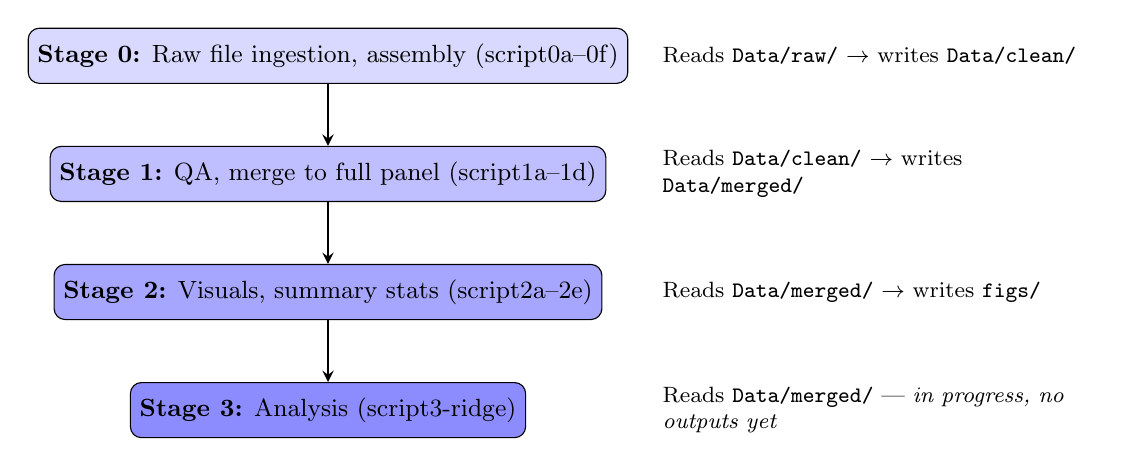
\begin{tikzpicture}[node distance=1.5cm, auto, font=\small]
  \node[draw, rounded corners, fill=blue!15, minimum width=3.5cm, minimum height=0.7cm] (s0) {\textbf{Stage 0:} Raw file ingestion, assembly (script0a--0f)};
  \node[draw, rounded corners, fill=blue!25, minimum width=3.5cm, minimum height=0.7cm, below of=s0] (s1) {\textbf{Stage 1:} QA, merge to full panel (script1a--1d)};
  \node[draw, rounded corners, fill=blue!35, minimum width=3.5cm, minimum height=0.7cm, below of=s1] (s2) {\textbf{Stage 2:} Visuals, summary stats (script2a--2e)};
  \node[draw, rounded corners, fill=blue!45, minimum width=3.5cm, minimum height=0.7cm, below of=s2] (s3) {\textbf{Stage 3:} Analysis (script3-ridge)};
  \draw[arrow] (s0) -- (s1);
  \draw[arrow] (s1) -- (s2);
  \draw[arrow] (s2) -- (s3);
  \node[right of=s0, xshift=5.5cm, text width=5.5cm, font=\footnotesize] {Reads \texttt{Data/raw/} $\rightarrow$ writes \texttt{Data/clean/}};
  \node[right of=s1, xshift=5.5cm, text width=5.5cm, font=\footnotesize] {Reads \texttt{Data/clean/} $\rightarrow$ writes \texttt{Data/merged/}};
  \node[right of=s2, xshift=5.5cm, text width=5.5cm, font=\footnotesize] {Reads \texttt{Data/merged/} $\rightarrow$ writes \texttt{figs/}};
  \node[right of=s3, xshift=5.5cm, text width=5.5cm, font=\footnotesize] {Reads \texttt{Data/merged/} — \textit{in progress, no outputs yet}};
\end{tikzpicture}
\end{center}

\end{frame}


\begin{frame}{Script pipeline: helpers}

The github repo, \texttt{mentalhealth} contains all of the scripts directly (no scripts execute from subfolders), that are needed to run project start to finish. Each script is clearly labeled. Two \textbf{key utility scripts} exist with helper functions used in multiple scripts. These include: 
\begin{itemize}
    \item[1] \texttt{packages.py} sets all packages that are necessary for analysis, has all shared import/export locations and other Dropbox path roots (interim-data, QA outputs, allegra-dropbox-copy for manual inspections)
    \item[2] \texttt{functions.py} provides FIPS normalization, CSV fallback readers, API wrappers, and the \texttt{latest\_files\_by\_descriptor()} selector used in Stage 1.
\end{itemize}
    
\end{frame}

% ─────────────────────────────────────────────────────────────────────────────
%  SECTION 4: SOURCE-BY-SOURCE CLEANING DETAIL
% ─────────────────────────────────────────────────────────────────────────────

\begin{frame}{script0a: Population + FIPS Panel}\label{0a}
\textbf{Purpose:} Build a complete annual FIPS-year population panel from 1990--2024 using four census vintages. Census vintages come in 10 year intervals (1990-2000, 2000-2010, etc.) So we use three 10-year cycles and then 2020-25 data. FIPS are provided on a census year basis, same 10-year interval update. 

\vspace{0.5em}
\textbf{Inputs:} \texttt{Data/raw/population/*.csv} (4 Census files) and \texttt{Data/raw/fips/foruse\_*.txt} (pipe/comma/whitespace delimited crosswalks)

\vspace{0.3em}
\textbf{Output:} \texttt{Data/clean/YYYY-MM-DD\_population\_full.csv} — \textbf{100\% county-year coverage}, used as second-best source population denominator throughout the project.

\end{frame}

\begin{frame}{script0a: Population + FIPS Panel}
\vspace{0.5em}
\textbf{Key cleaning steps:}
\begin{enumerate}\small
    \item Reads each Census file by fragment name match (\texttt{cc-est2024}, \texttt{cc-est00int-tot}, etc.) — \textbf{if filenames change, these fragment strings must be updated}
    \item Identifies FIPS crosswalk delimiters via \texttt{sniff\_delimiter()} and reads accordingly (pipe / comma / fixed-width)
    \item Expands each decade's crosswalk to annual rows via \texttt{expand\_years\_cross()}
    \item \textbf{Hardcoded manual fix:} FIPS 12025 $\rightarrow$ 12086 (Miami-Dade) and two counties added for 1990 (Yellowstone NP \texttt{30113}, South Boston \texttt{51780})
    \item Drops state-level summary rows where \texttt{county == state}
    \item Normalizes DC to \texttt{11001}; drops non-US state codes; deduplicates on \texttt{(fips, year)} keeping last (QA shows no dupes exist, one FIPS per year per county name)
\end{enumerate}
\end{frame}


\begin{frame}{script0b: USDA NASS Agriculture (CAFO)}\label{0b}

\textbf{Purpose:} Pull all agriculture operation counts by animal and size class from USDA NASS Quick Stats API (census years: 2002, 2007, 2012, 2017). Agriculture operations include any farming (non-processing or slaughter) establishment, and is classified by type of animal and purpose of breeding (i.e. cattle for milk vs. beef). 


\textbf{Inputs:} Census API. Where API doesn't work, we use pre-downloaded \texttt{.dta} files as previously saved in \texttt{Data/raw/usda/*.dta}

\vspace{0.3em}
\textbf{Outputs:} \texttt{*\_cafo\_ops\_by\_size\_compact.csv} (pivot: county $\times$ year $\times$ commodity $\times$ small/medium/large), establishment counts at county-level are intergrated into \texttt{merged\_all.csv}

\end{frame}


\begin{frame}{script0b: USDA NASS Agriculture (CAFO)}
\vspace{0.3em}
\textbf{Key assumptions, data cleaning step 1: }
\begin{itemize}\small
    \item \textbf{API key:} \texttt{os.environ["USDA\_NASS\_API\_KEY"] = "30643212-..."} — \textbf{must be changed per user}
    \item \textbf{API fallback:} If API fails, reads \texttt{.dta} files from \texttt{Data/raw/usda/}
    \item \textbf{backfill for non-census years}. Using the previous four years, we use non-transformed backfilled data from most recent census year to fill in for annual basis.
    \item Filters to: \texttt{CENSUS} source, \texttt{COUNTY} level, animals = \{CATTLE, CHICKENS, HOGS\}, unit = \{HEAD, OPERATIONS\}
    \item Splits queries $>50{,}000$ rows by domain to avoid API limits (rate sleep: 0.4s)
\end{itemize}

\end{frame}

\begin{frame}{script0b: USDA NASS Agriculture (CAFO)}

\textbf{Data creation: Size classification thresholds for CAFOs}: Using the USDA CAFO definition (on animal head count parameter only), applied per inventory bin code. Note the bins are a translation of \textit{ranges} of number of animal heads.

\vspace{2em}

\begin{center}
  \begin{tblr}{colspec={Q[l,2.5cm] Q[c,3cm] Q[c,3cm]}, hlines, vlines, row{1}={font=\bfseries\small}, row{2-Z}={font=\small}}
Animal & Medium $\geq$ bin & Large $\geq$ bin \\
Broiler chickens & 3 & 5 \\
Layer chickens & 7 & 9 \\
Cattle / Hogs & 6 & 7 \\
\end{tblr}

\end{center}

\end{frame}



\begin{frame}{script0c: Health Data (CHR + CDC Mortality)}\label{0c}

\textbf{Purpose:} Clean County Health Rankings (CHR) mental health surveys and CDC deaths-of-despair county files; merge into a single health panel.

\vspace{0.3em}

\textbf{Inputs:} CHR mental health survey data found in \texttt{Data\_mental\_analytic*.csv}. These are merged. Then CDC data exported from WONDER as saved in \texttt{Data\_cdc\_cty-level-deathsofdespair*.csv}.

\vspace{0.3em}

\textbf{Outputs:} Clean mental health survey data in \texttt{*\_mentalhealthrank\_full.csv}, \texttt{*\_cdc\_county\_year\_deathsofdespair.csv}, \\
\textbf{depreciated output:} \texttt{*\_mh\_mortality\_fips\_yr.csv}
\end{frame}


\begin{frame}{script0c: Health Data (CHR + CDC Mortality)}

\textbf{CHR cleaning (Pass 1):}
\begin{itemize}\small
    \item Year inferred from filename via regex from the 4-digit year (on all files)
    \item Column names normalized: lowercased, special characters stripped, label drift harmonized (e.g.\ \texttt{limited access to healthy foods} $\rightarrow$ \texttt{access to healthy foods})
    \item Duplicate columns resolved by keeping the most complete version (highest fill rate)
    \item \textbf{Variable selection thresholds:} include if present in $\geq 11$ annual files (majority rule) OR $\geq 8$ files with $\geq 80\%$ average fill
    \begin{itemize}
        \item[a] Threshold can be changed in the script
        \item[b] Conservative threshold chosen first
    \end{itemize}
\end{itemize}

\end{frame}


\begin{frame}{script0c: Health Data (CHR + CDC Mortality)}

\textbf{CDC cleaning (Pass 2):}
\begin{itemize}\small
    \item Reads files matching \texttt{cty-level-deathsofdespair-YYYY.csv} from \texttt{Data/raw/cdc/}
    \item Parses: deaths, population, crude rate, \texttt{is\_unreliable} flag (from ``unreliable'' / ``suppressed'' in notes)
    \item \textbf{Suppression caveat:} crude rate is missing for \textasciitilde85--93\% of rural county-years (CDC suppresses when deaths $< 10$). Raw death count is always retained.
    \item Using the population data from \texttt{script1a-pop-fips.py} we can calculate the incident rate of deaths
    \item Note: missing values from CDC are assumed to be missing data, and are kept separate from values classified as zero. QA check performed to ensure mislabeling does not occur. 
\end{itemize}

\textbf{Merge:} Outer join of CHR + CDC on \texttt{(fips, year)}; validated as 1:1. 
\end{frame}




\begin{frame}{script0d: Crime Data (FBI UCR)}\label{0ad}
\textbf{Purpose:} Stack annual FBI UCR incident files as provided from 2023 analysis (precinct $\rightarrow$ county aggregation). Then we select violent crime columns (researcher discretion), and collapse the number of incidence to FIPS-year counts.

\vspace{0.3em}
\textbf{Inputs:} Loads all \texttt{.csv} from \texttt{Data/raw/crime/total-v1/} (\textasciitilde 7 GB combined in memory — beware on low-RAM machines)
%\textbf{Hardcoded paths:} \texttt{interim\_override} in script — update per user. 
\\
\vspace{0.3em}
\textbf{Outputs:} \texttt{*\_crime\_fips\_level\_final.csv} (main), \texttt{*\_crime\_demog\_final.csv} (with demographics)

\end{frame}


\begin{frame}{script0d: Crime Data (FBI UCR)}

\textbf{Key steps:}
\begin{enumerate}\small
    \item \textbf{Crime types} selected by research team: aggravated assault, DUI, fondling, incest, intimidation, kidnapping, rape, sexual assault, simple assault, statutory rape, human trafficking (commercial sex + involuntary servitude)
    \item Column normalization: unicode dash normalization, whitespace collapse, then fuzzy matching for human trafficking columns (some encoding issues required manual rename map)
    \item Collapses first to \texttt{(fips, year, sex, race, ethnicity)} keys, then \textbf{further to \texttt{(fips, year)} only} for the main panel
    \item \textbf{Optional disaggregation extension} (off by default): set env var \texttt{RUN\_CRIME\_DISAGG\_EXTENSION=1} to produce sex/age/race breakdowns in \texttt{interim-data/crime-disagg-extension/}
\end{enumerate}
\end{frame}



\begin{frame}{script0e: NCHS Urban-Rural Classification}\label{0e}

\textbf{Purpose:} Build an annual rural/urban classification panel from the NCHS 6-level code scheme, used to define the analytical sample. Panel restricted to years $\geq$ 2000. \\
\vspace{0.3em}

\textbf{Inputs:} Using \texttt{Data/raw/nchs/NCHSurb-rural-codes.csv}, containing \texttt{year x county} codes for given base years (1990, 2006, 2013, 2023).
\\
\vspace{0.3em}

\textbf{Output:} \texttt{YYYY-MM-DD-rural-key.csv} — the filter applied in \texttt{script1c} to drop all non-rural counties before creating \texttt{YYYY-MM-DD-final-merge.csv}
\end{frame}

\begin{frame}{script0e: NCHS Urban-Rural Classification}
\textbf{NCHS 6-level scheme:}
\vspace{0.3em}
\begin{center}
    
\begin{tblr}{colspec={Q[c,1.5cm] Q[l,4.5cm] Q[c,3cm]}, hlines, vlines, row{1}={font=\bfseries\small}, row{2-Z}={font=\small}}
Code & Label & non\_large\_metro \\
1 & Large central metro & \textbf{0 (excluded)} \\
2 & Large fringe metro & \textbf{0 (excluded)} \\
3 & Medium metro & 1 (included) \\
4 & Small metro & 1 (included) \\
5 & Micropolitan & 1 (included) \\
6 & Noncore (rural) & 1 (included) \\
\end{tblr}

\end{center}

\end{frame}


\begin{frame}{script0e: NCHS Urban-Rural Classification}

Data manipulation for this dataset is simple. No changes to data structure are needed. Backfilling for missing years (non-recorded years) are needed. 

\vspace{0.3em}

\textbf{Annual expansion logic:} NCHS provides codes at four base years. Each base year is forward-filled to cover the next period:
\begin{itemize}\small
    \item 1990 code $\rightarrow$ 1990--2005; 
    \item 2006 code $\rightarrow$ 2006--2012; 
    \item 2013 code $\rightarrow$ 2013--2022; 
    \item 2023 code $\rightarrow$ 2023
\end{itemize}
\end{frame}

\begin{frame}{script0f: FSIS processing establishments pipeline}\label{0f}

\textbf{Purpose:} Multi-step pipeline to clean FOIA-requested FSIS inspection data, recover missing FIPS codes for establishments in the FSIS data via the HUD ZIP-to-FIPS crosswalk, and create a \texttt{county x year} dataframe of inspected facilities. \\
\vspace{0.3em}
\textbf{Requirements:} \texttt{HUD\_API\_TOKEN} env var required (unless \texttt{--hud-strategy skip}). \\
\vspace{0.3em}
%\textbf{Coverage note:} FSIS data is \textbf{2017 only} — usable for cross-section analysis only, not panel. \\
\vspace{0.3em}
\textbf{Output:} \texttt{*\_fsis\_county\_year\_fips\_est\_size\_type\_summary\_hudbulk\_manualzip.csv}, and inclusion in FSIS facilities into final merged panel

\end{frame}


\begin{frame}{script0f: FSIS processing establishments pipeline}
\textbf{Pipeline sub-scripts (run in order):}
\begin{enumerate}\small
    \item \texttt{script0e-fsis-slaughterhouses.py} — extract raw FSIS inspection records
    \item \texttt{script0h-fsis-establishment-size-panel.py} — build establishment × size panel
    \item \textbf{HUD fill} (choose strategy via \texttt{--hud-strategy}):
    \begin{itemize}
        \item \texttt{bulk} (default): ZIP-to-FIPS crosswalk for all establishments with city/state/ZIP
        \item \texttt{targeted}: only missing establishments
        \item \texttt{skip}: no HUD fill
    \end{itemize}
    \item \texttt{script0l} — apply manual ZIP template (if present in \texttt{qa-fsis/})
    \item \texttt{script0m} — deterministic FIPS completion
    \item \texttt{script0n} — apply manual county labels (if present)
\end{enumerate}
\end{frame}

% ─────────────────────────────────────────────────────────────────────────────
%  SECTION 5: MASTER MERGE (script1c)
% ─────────────────────────────────────────────────────────────────────────────

\section{Merging into the panel}

\begin{frame}{script1c: The master merge file}
\textbf{Purpose:} Combine all clean source files into one county-year panel, restricted to rural counties, with all iterated or re-calculated columns for analysis.

\vspace{0.3em}
\textbf{Step-by-step logic:}
\begin{enumerate}\small
    \item \textbf{Auto-selects latest files} from \texttt{Data/clean/} by descriptor string (date prefix stripped)
    \item \textbf{Builds rural allowed-keys:} reads \texttt{*-rural-key.csv}, keeps only \texttt{(fips, year)} where \texttt{non\_large\_metro == 1}
    \item \textbf{Base panel:} CAFO compact file reduced to one row per \texttt{(fips, year)} — numeric columns summed (\texttt{min\_count=1} to preserve NaN for all-missing groups); text columns take first observed value
    \item \textbf{CAFO animal $\times$ size block:} pivot adds columns \texttt{cafo\_\{cattle/hogs/chickens\}\_\{small/medium/large\}}, \texttt{cafo\_total\_ops\_all\_animals}, \texttt{cafo\_total\_ops\_chickens}
\end{enumerate}
\end{frame}

\begin{frame}{script1c: The master merge file}
Cont'd \textbf{step-by-step logic}:
\begin{enumerate}
    \item[5] \textbf{Left-joins} CDC mortality, crime, FSIS, CHR mental health, and population onto the rural CAFO base frame. 
    \begin{itemize}
        \item \textit{Note: Final QA is needed to ensure  rural county dataframe is used as base, not CAFO dataframe, so we don't exclude zero-presence of ag activity counties}. 
    \end{itemize}
    \item[6] \textbf{Derived crude rate:} \texttt{crude\_rate\_from\_census\_pop} = deaths / census population $\times$ 100{,}000 — computed only where deaths $> 0$ and population $> 0$. This is done for $crude_rate$ mortality data flagged as unreliable in source file. 
    \item[7] \textbf{Missingness flags:} \texttt{cdc\_in\_query}, where \texttt{deaths\_is\_zero} flag captures missing CDC data. CDC returned 0 deaths — ambiguous, rate set to NaN. 
\end{enumerate}
\end{frame}

\begin{frame}{script1c: Assumptions \& caveats}
\begin{itemize}
    \item \textbf{Rural filter is the primary sample restriction.} Large central and fringe metro counties are dropped entirely.
    \item \textbf{Column naming convention:} All merged columns are suffixed with the descriptor of their source file (e.g.\ \texttt{population\_population\_full}). Do not rename these manually.
    \item \textbf{Summing with \texttt{min\_count=1}:} When collapsing duplicates, numeric columns are summed but an all-missing group is preserved as NaN rather than coerced to 0.
    %\item \textbf{Ambiguous CDC zeros:} \texttt{deaths\_is\_zero == 1} does not necessarily mean true zero deaths — could be suppression artefact. The crude rate is set to NaN for these rows. Do not treat them as confirmed no-death counties.
    %\item \textbf{FSIS joins on year = 2017 only:} FSIS establishments appear only for 2017. All other years will have NaN in FSIS columns — this is expected.
    \item \textbf{Text column resolution:} String columns from multi-row sources take the \textit{first} non-null observed value after the rural filter. This is appropriate for geographic labels, not used for time-varying text fields.
\end{itemize}
\end{frame}

% ─────────────────────────────────────────────────────────────────────────────
%  SECTION 6: DERIVED VARIABLES & QA (script1d, script1e)
% ─────────────────────────────────────────────────────────────────────────────

\begin{frame}{script1e: Derived variables (CHR counts + ratio flags)}
\textbf{Purpose:} Two-pass augmentation of the merged panel using County Health Rankings (CHR) data. Recall the CHR data is survey data at the county level. The data provides raw data, crude rates of incidence, numerator, denominator and confidence intervals (CIs). CIs cannot be used, but to calculate crude rates, we use population in the panel key for consistency in calculations. 

\textbf{Output:} \texttt{*\_full\_merged\_derived.csv} (original panel unchanged). Note, in the most recent version of the code, this has been dropped and now \texttt{*\_full\_merged.csv} contains the changes made in this script. 
\end{frame}


\begin{frame}{script1e: Derived variables (CHR counts + ratio flags)}
\vspace{0.5em}
\textbf{Pass 1: Impute counts for rate-only CHR variables:}
\begin{itemize}\small
    \item Applies to 6 variables that have \texttt{raw\_value} only (no numerator column): frequent mental distress, frequent physical distress, insufficient sleep, access to exercise, \% American Indian/Alaskan Native, \% non-Hispanic African American
    \item Formula: \texttt{count\_imputed = (raw\_value / 100) $\times$ census\_population}
    \item Scale auto-detected: median $\leq 1$ $\Rightarrow$ proportion (multiply by 100); otherwise already a percentage
    \item \textbf{These are imputed, not measured counts.} Label: \texttt{*\_count\_imputed}
\end{itemize}

\end{frame}


\begin{frame}{script1e: Derived variables (CHR counts + ratio flags)}

\textbf{Pass 2: Verify numerator/denominator consistency:}
\begin{itemize}\small
    \item For all CHR variables with both \texttt{numerator} and \texttt{denominator} columns, checks: \texttt{numerator / denominator $\approx$ raw\_value}
    \item Tolerance: absolute diff $>$ 0.05 (5 pp) OR relative diff $>$ 10\% $\Rightarrow$ flagged
    \item Flag column: \texttt{*\_ratio\_flag = 1}. Variables with $>5\%$ rows flagged generate a warning.
    \item \textbf{No values are modified} — flags only. Inspect flagged variables before use in regression.
\end{itemize}
\textit{$\Rightarrow$ we find no issue with data assembly by CHR. Survey method does not yield obvious issues or column discrepencies.}
\end{frame}

\begin{frame}{script1e + 1c: Derived variables (CHR counts + incidence rates standardization)}


\textbf{Pass 3: Build standard incidence rates to per 100k rate:}
\begin{itemize}\small
    \item  The incidence rates in the CHR data are reported with different denominators
    \item In \texttt{script1c} we align crime and health data on rates of incidence for comparison
    \item Incidence rate columns are pulled from CHR data, and dependeing on presentation, are converted. \hyperlink{incidence-rate-calc}{\beamerbutton{See details in appendix}}
    \end{itemize}
\end{frame}

\begin{frame}{script1d: CDC crude rate sense check (population)}

\textbf{Purpose:} Validate that CDC-reported crude rates align with rates recomputed from merged deaths and census population. Flags systematic discrepancies.

\vspace{0.3em}
\textbf{Diagnostics produced:}
\begin{itemize}\small
    \item \texttt{crude\_rate\_recalc\_census\_pop} = deaths / census pop $\times$ 100{,}000 (recomputed)
    \item \texttt{crude\_rate\_recalc\_cdc\_pop} = deaths / CDC pop $\times$ 100{,}000 (internal check)
    \item \texttt{diff\_census\_minus\_cdc}: difference between recomputed and CDC-reported rates
    \item \texttt{z\_diff\_from\_zero\_sd}: standardized distance of discrepancy from zero
    \item \texttt{population\_pct\_diff\_census\_vs\_cdc}: \% difference between Census and CDC population denominators
\end{itemize}
\end{frame}

\begin{frame}{script1d: CDC crude rate sense check (population)}


\textbf{QA outputs} (saved to \texttt{Data/merged/figs/panel-sumstats-by-farms/}):
\begin{itemize}\small
    \item \texttt{*\_qa\_cdc\_cruderate\_sensecheck\_overall.csv} — global summary statistics
    \item \texttt{*\_qa\_cdc\_cruderate\_sensecheck\_by\_year.csv} — year-by-year breakdown
    \item \texttt{*\_qa\_cdc\_cruderate\_sensecheck\_outliers\_top1000.csv} — largest discrepancies
\end{itemize}

\vspace{0.3em}
{\small Note there are \textbf{hardcoded paths in this script:} \texttt{MERGED\_DIR} and \texttt{OUT\_QA\_DIR} are absolute paths — update before running on a new machine.} \\

\vspace{0.3em}
{\small \textbf{Population comparison} demonstrated CDC, CHR and US census population data was not different enough to flag between sources.}
\end{frame}


% ─────────────────────────────────────────────────────────────────────────────
%  SECTION 7: THE FINAL MERGED PANEL
% ─────────────────────────────────────────────────────────────────────────────
\section{Review of panel dataset}


\begin{frame}{Merged panel: what is it?}
Recall our final \textbf{file:} \texttt{Data/merged/YYYY-MM-DD\_full\_merged.csv}

\vspace{0.5em}
\textbf{Unit of observation:} county-year (\texttt{fips}, \texttt{year})



\textbf{Sample restriction:} non-large-metro counties only (\texttt{non\_large\_metro == 1}) for 2,314 counties per year 

\textbf{Year range:} \textasciitilde2000--2023 (source-dependent). 2010-2020 offers most complete set of data from mental health survey, crime and agriculture data. See \texttt{YYYY-MM-DD\_full\_merged\_2010-\_2020.csv}

\textbf{Panel structure:} unbalanced — not all sources cover all years. In total: we have 65,828 rows and 2,879 unique (rural) counties.



\end{frame}


\begin{frame}{Merged panel: what is it?}
\textbf{Column naming convention:}

All non-key columns are suffixed with their source descriptor:
\begin{itemize}\small
    \item \texttt{..\_cafo\_ops\_by\_size\_compact} — CAFO columns
    \item \texttt{..\_cdc\_county\_year\_deathsofdespair} — CDC mortality
    \item \texttt{..\_mentalhealthrank\_full} — CHR survey
    \item \texttt{..\_crime\_fips\_level\_final} — UCR crime
    \item \texttt{..\_fsis\_county\_year\_..\_summary\_..} — FSIS plants
    \item \texttt{..\_population\_full} — Census population
\end{itemize}
\end{frame}


\begin{frame}{Key variables of interest(1/2)}
\begin{tblr}{
  colspec = {Q[l,3.7cm] Q[l,5cm] Q[l,3.2cm]},
  hlines, vlines,
  row{1} = {font=\bfseries\small},
  row{2-Z} = {font=\footnotesize},
}
Variable & Description & Source \\
\texttt{cafo\_\{animal\}\_\{size\}} & Count of small/medium/large CAFO ops by animal type (cattle, hogs, chickens) & USDA NASS census years \\
\texttt{cafo\_total\_ops\_all} \texttt{\_animals} & Total CAFO operations across all animal types & Derived in script1c \\
\texttt{population\_} \texttt{population\_full} & Annual county population (Census) & script0a — 100\% coverage \\
\texttt{deaths\_cdc\_...} & Raw deaths-of-despair count & CDC WONDER \\
\texttt{crude\_rate\_cdc\_...} & CDC-reported crude rate (suppressed $<10$ deaths) & CDC WONDER \\
\end{tblr}
\end{frame}


\begin{frame}{Key variables of interest (2/2)}
\begin{tblr}{
  colspec = {Q[l,3.7cm] Q[l,5cm] Q[l,3.2cm]},
  hlines, vlines,
  row{1} = {font=\bfseries\small},
  row{2-Z} = {font=\footnotesize},
}
\texttt{crude\_rate\_} \texttt{from\_census\_pop} & Recomputed crude rate using Census pop denominator & Derived in script1c \\
\texttt{cdc\_in\_query} & 1 if county-year appeared in CDC WONDER download & Derived flag \\
\texttt{deaths\_is\_zero} & 1 if CDC returned Deaths=0 (ambiguous) & Derived flag \\
\texttt{poor\_mental\_health} \texttt{\_days\_raw\_value\_...} & Avg days/month of poor mental health (CHR) & County Health Rankings \\
\texttt{frequent\_mental\_} \texttt{distress\_raw\_value\_...} & \% adults with frequent mental distress (CHR) & County Health Rankings \\
\texttt{n\_unique\_establishments} \texttt{\_fsis\_...} & Count of FSIS-regulated plants per county (2017 only) & USDA FSIS FOIA \\
\texttt{aggravated\_assault} \texttt{\_crime\_...} & UCR aggravated assault count & FBI UCR \\
\end{tblr}
\end{frame}



\begin{frame}{Key variables of interest: coverage (1/2)}
\begin{tblr}{
  colspec = {Q[l,4cm] Q[c,2.5cm] Q[c,2.5cm] Q[l,3cm]},
  hlines, vlines,
  row{1} = {font=\bfseries\small},
  row{2-Z} = {font=\small},
}
Source & Year range & Fill (\% panel) & Notes \\
Census population & 1990--2024 & $\approx$ 100\% & Used as denominator \\
CAFO operations & 2002, 2007, 2012, 2017, 2022 & $\approx$ 97\% (census yrs) & Census years only \\
CHR poor mental health days & 2004--2022 & $\approx$ 90\% (2010+) & Usable 2010 onward \\
CHR frequent mental distress & 2016--2022 & $\approx$ 90\% (2016+) & Not for pre-2016 panel \\
CHR excessive drinking & 2011--2022 & $\approx$ 80\% (2011+) & Full from 2016 \\
\end{tblr}
\end{frame}

\begin{frame}{Key variables of interest: coverage (2/2)}
\begin{tblr}{
  colspec = {Q[l,4cm] Q[c,2.5cm] Q[c,2.5cm] Q[l,3cm]},
  hlines, vlines,
  row{1} = {font=\bfseries\small},
  row{2-Z} = {font=\small},
}
CDC deaths of despair (raw count) & 1999--2020 & Varies & Count retained always \\
CDC crude rate & 1999--2020 & $<$ 15\% & Suppressed $<10$ deaths \\
FBI UCR crime & \textasciitilde 2000--2022 & Varies by year & Violent crime subset \\
FSIS establishments & \textbf{2017 only} & 2017 cross-section & Cross-section use only \\
\end{tblr}

\vspace{0.5em}
{\footnotesize \textbf{Recommended panel window for outcome analysis: 2010--2015.} This balances CHR mental health coverage ($\approx$90\%), CAFO census year availability (2012), and pre-FSIS comparability.}
\end{frame}

\begin{frame}{Data quality issues}
\textbf{Known issues and how to handle them:}

\vspace{0.5em}
\begin{enumerate}
    \item \textbf{CDC crude rate missingness ($\approx$85--93\%):} This is by design — CDC suppresses for $<10$ deaths. Use raw death counts or the recomputed \texttt{crude\_rate\_from\_census\_pop} for analysis. Flag \texttt{cdc\_in\_query = 0} means the county-year was absent from the CDC WONDER pull entirely.

  %  \item \textbf{FSIS data is 2017 cross-section only:} All panel years outside 2017 will be NaN in FSIS columns. Do not interpret as ``zero plants.'' Use a binary indicator or restrict to 2017.

    \item \textbf{CAFO data at census years only (2002, 2007, 2012, 2017, 2022):} Interpolating between census years requires justification in explanation. 

\end{enumerate}
\end{frame}

\begin{frame}{Data quality issues}
\textbf{Known issues and how to handle them:}

\vspace{0.5em}
\begin{enumerate}
    \item \textbf{CHR \texttt{frequent\_mental\_distress} starts 2016:} Cannot be used in a pre-2016 panel. Use \texttt{poor\_mental\_health\_days} (available from \textasciitilde 2004, reliable from 2010) as the primary mental health outcome for longer panels.

    \item \textbf{CAFO per-capita transformation:} Raw CAFO operation counts are heavily right-skewed. For scatter plots and regressions, use \texttt{log(cafo\_total\_ops\_all\_animals / population $\times$ 10{,}000 + 1)}.
\end{enumerate}
\end{frame}

\begin{frame}{Time-dependent slices}
\begin{tblr}{
  colspec = {Q[l,5cm] Q[l,4cm] Q[l,3cm]},
  hlines, vlines,
  row{1} = {font=\bfseries\small},
  row{2-Z} = {font=\small},
}
File suffix & Year range & Recommended use \\
\texttt{\_full\_merged.csv} & All years (rural) & Starting point for all analysis \\
\texttt{\_full\_merged\_2005\_2010.csv} & 2005--2010 & Pre-recession window \\
\texttt{\_full\_merged\_2010\_2020.csv} & 2010--2020 & \textbf{Recommended primary panel} \\
\texttt{\_full\_merged\_census\_years.csv} & 2002, 2005, 2007, 2012, 2017, 2022 & CAFO-aligned cross-sections \\
\texttt{\_full\_merged\_derived.csv} & All years + derived & CHR imputed counts + ratio flags \\
\end{tblr}
\end{frame}

\begin{frame}[fragile]{Using the data}

\textbf{How to load the latest panel in Python:}

\begin{lstlisting}
from functions import latest_file_glob
import pandas as pd

merged_dir = "~/Dropbox/Mental/Data/merged"
path = latest_file_glob(merged_dir, "*_full_merged.csv")
df = pd.read_csv(path, low_memory=False)

# Always normalize the key after loading:
from functions import normalize_panel_key
df = normalize_panel_key(df, dropna=True)
\end{lstlisting}

\end{frame}

% ─────────────────────────────────────────────────────────────────────────────
%  SECTION 8: HARDCODED PATHS REFERENCE
% ─────────────────────────────────────────────────────────────────────────────

\section{Appendix}

\begin{frame}{Hardcoded paths}
\textbf{Before running any script on a new machine, update the following:}

\vspace{0.5em}
\begin{tblr}{
  colspec = {Q[l,3cm] Q[l,5cm] Q[l,4cm]},
  hlines, vlines,
  row{1} = {font=\bfseries\small},
  row{2-Z} = {font=\footnotesize},
}
Script & Variable / Line & What to change \\
\texttt{packages.py} & \texttt{db\_base = os.path.expanduser("$\sim$/Dropbox/Mental")} & Dropbox root path \\
\texttt{script0a, 0b, 0d} & \texttt{repo = "/Users/allegrasaggese/Documents/..."} & GitHub repo path \\
\texttt{script0b} & \texttt{USDA\_NASS\_API\_KEY} env var & Personal API key \\
\texttt{script0b} & \texttt{donor\_path = ".../2026-02-23\_ag\_annual\_df.csv"} & Backfill CSV path \\
\texttt{script0d} & \texttt{interim\_override = "/Users/allegrasaggese/Dropbox/..."} & Local Dropbox copy path \\
\texttt{script0f} & \texttt{HUD\_API\_TOKEN} env var & HUD API token \\
\texttt{script1d} & \texttt{MERGED\_DIR}, \texttt{OUT\_QA\_DIR} & Absolute output paths \\
\end{tblr}

\vspace{0.5em}
{\footnotesize \textbf{Best practice:} Set \texttt{db\_base} in \texttt{packages.py} to the correct Dropbox root for your machine. All other paths are derived from \texttt{db\_base} via \texttt{os.path.join()} and will resolve automatically once this is set correctly.}
\end{frame}

\begin{frame}{CHR conversions for incidence rates}\label{incidence-rate-calc}
In the County Health Survey (CHR) data, variables are recorded with different \textit{rates of incidence}. See table below for steps to convert to same incidence rate (per 100,000 people). 

\begin{table}[h]
\centering
\small
\begin{tblr}{
  colspec = {Q[l,3.2cm] Q[l,8.2cm] Q[c,2cm]},
  hlines, vlines,
  row{1} = {font=\bfseries},
}
Current unit & Variables & Conversion \\
Proportion (0--1) &
  All \texttt{\%\_*}, \texttt{excessive\_drinking}, \texttt{adult\_obesity},
  \texttt{adult\_smoking}, \texttt{unemployment}, \texttt{uninsured},
  \texttt{low\_birthweight}, \texttt{children\_in\_poverty}, etc. &
  $\times$ 100{,}000 \\
Per 1{,}000 &
  \texttt{infant\_mortality}, \texttt{teen\_births} &
  $\times$ 100 \\
Per 10{,}000 &
  \texttt{social\_associations} &
  $\times$ 10 \\
\end{tblr}
\end{table}
\end{frame}


\begin{frame}{CHR conversions for incidence rates}
\textit{Cont'd table:}

\begin{table}[h]
\centering
\small
\begin{tblr}{
  colspec = {Q[l,3.2cm] Q[l,8.2cm] Q[c,2cm]},
  hlines, vlines,
  row{1} = {font=\bfseries},
}
Current unit & Variables & Conversion \\
Already per 100{,}000 &
  \texttt{violent\_crime}, \texttt{homicides},
  \texttt{motor\_vehicle\_crash\_deaths}, \texttt{injury\_deaths},
  \texttt{hiv\_prevalence}, \texttt{STIs},
  \texttt{premature\_age-adjusted\_mortality}, \texttt{child\_mortality},
  \texttt{preventable\_hospital\_stays},
  \texttt{on-road MVC ER visits} &
  no change \\
Provider ratio (providers/person) &
  \texttt{primary\_care\_physicians}, \texttt{dentists},
  \texttt{mental\_health\_providers},
  \texttt{other\_primary\_care\_providers} &
  $\times$ 100{,}000 \\
\end{tblr}
\label{tab:chr-conversions2}
\end{table}
\end{frame}


\begin{frame}{CHR conversions for incidence rates}
\textit{Cont'd table:}

\begin{table}[h]
\centering
\small
\begin{tblr}{
  colspec = {Q[l,3.2cm] Q[l,8.2cm] Q[c,2cm]},
  hlines, vlines,
  row{1} = {font=\bfseries},
}
Current unit & Variables & Conversion \\
Not a rate --- leave as-is &
  \texttt{poor\_mental\_health\_days} (avg days/month),
  \texttt{poor\_physical\_health\_days},
  \texttt{income\_inequality} (Gini),
  \texttt{food\_environment\_index},
  \texttt{air\_pollution} PM ($\mu$g/m$^3$),
  \texttt{median\_household\_income},
  \texttt{premature\_death} (YPLL per 100k --- already standardized),
  \texttt{poor\_or\_fair\_health} &
  --- \\
\end{tblr}
\label{tab:chr-conversions3}
\end{table}
    
\end{frame}

\begin{frame}{CHR conversions for incidence rates}
Conversions were done for mental health variables to make them \textbf{comparable} numerically. Incidence per 100,000 is also how crime data is reported, and therefore this cleaning standardizes the process. \\
\vspace{2mm}

The rate standardization is in \texttt{script1c-merge-dataclean.py}, lines $\sim$489–565, in a block called \texttt{\# Rate Standardization}. Within the merge dataset, we build the incidence data.                                         
\end{frame}


\begin{frame}{CHR conversions for incidence rates: step by step}
    \begin{itemize}
    \item \textbf{Part 1} crime counts $\rightarrow$ per 100k: detects all columns ending in \texttt{\_crime\_fips\_level\_final}, divides by \texttt{population\_population\_full × 100,000}, writes \texttt{*\_per100k} columns. 13 crime variables exist.  
    \item \textbf{Part 2} CHR variables $\rightarrow$ per 100k: four explicit lists, each with a known multiplier (see previous table):
    \begin{enumerate}
        \item Provider ratios (raw ratio like 0.0005) × 100,000 $\rightarrow$ e.g. \texttt{primary\_care\_physicians\_per100k}
        
        \item Per-1,000 vars $\times$ 100 $\rightarrow$ \texttt{teen\_births\_per100k}, \texttt{infant\_mortality\_per100k}
        
        \item Per 10,000 vars $\times$ 10 $\rightarrow$ \texttt{social\_associations\_per100k}
        
        \item 27 proportion (0–1) vars $\times$ 100,000 $\rightarrow$ e.g. \texttt{adult\_obesity\_per100k} 
    \end{enumerate}
\end{itemize}   
\end{frame}



\end{document}